\documentclass[letterpaper,12pt]{extarticle}%Preambulo
\usepackage[utf8]{inputenc}%Preambulo
\usepackage[spanish,mexico]{babel}%Preambulo
\usepackage{ae}
\usepackage{amsmath,amssymb,amsfonts,latexsym,cancel}%Preambulo
\usepackage{hyperref}%Preambulo
\usepackage[pdftex]{graphicx}%Preambulo
\usepackage{wrapfig}%Preambulo
\usepackage[rflt]{floatflt}%Preambulo
\usepackage{fancyhdr}%%Pre?mbulo
\usepackage{mathptmx}%%Pre?mbulo
\usepackage{float}%%Pre?mbulo
\usepackage{longtable,multirow,booktabs}%%Pre?mbulo
%\usepackage{cite}
\usepackage{wrapfig}%%Pre?mbulo
\usepackage[rflt]{floatflt}%%Pre?mbulo
\usepackage{natbib} %%Pre?mbulo
\usepackage{multicol}%%Pre?mbulo
\usepackage{caption}%%Pre?mbulo
\usepackage{geometry}
\usepackage{wrapfig}
\usepackage{adjustbox}
\usepackage{amsmath}
\usepackage{parskip}
\usepackage{tikz}
\usepackage{lipsum}
\usepackage{xcolor}
\usepackage[T1]{fontenc}

\captionsetup{
       font=small,
       labelfont=bf,
       tableposition=top,
       hypcap=false
    }

\DeclareGraphicsExtensions{.pdf, .png, .jpg, .PNG, .JPG}%Cuando ponemos im?genes ya no es necesario poner la extensi?n

%%%FORMATO DE LA P?GINA%%%
\textheight = 21cm %Medidas de la  p?gina
\textwidth = 18cm  %Medidas de la p?gina
\topmargin = -1cm  %Medidas de la p?gina    
\oddsidemargin = -1cm %Medidas de la p?gina
\pagestyle{fancy} %Dise?o de la p?gina
\lhead{Universidad de la Sierra Sur}%%LeftHead
\chead{
\includegraphics[width=1cm, height=1cm]{imag//logL}}%%CenterHead
%\lfoot{USM}
\rhead{Licenciatura en Informática}%%RightHead
%\lfoot{Gonz?lez Chico Juan Daniel} %Pie de pagina izquierdo

\setlength{\columnsep}{7mm}%Comandos para el formato de la p?gina
%\setlength{\parindent}{4em}%Sangr?a al comenzar un nuevo p?rrafo
\setlength{\parindent}{0.5in}
%\setlength{\parindent}{4em}%Sangr?a al comenzar un nuevo p?rrafo
\setlength{\parskip}{1em}%distancia entre p?rrafos
\renewcommand{\baselinestretch}{1.0}% Espacio entre l?nea y l?nea
\setlength{\headheight}{33pt}

\hypersetup{
	colorlinks = true,
	linkcolor = black,
	urlcolor = cyan
}
\urlstyle{same}

\begin{document}

    \begin{titlepage}
		% Mine page for add image at scale with footer image in 
		\begin{figure}[ht]
		   \minipage{0.76\textwidth}
				
\includegraphics[width=4cm]{imag//logColor.jpg}
				\label{escudoFI}
		   \endminipage
		   \minipage{0.32\textwidth}

				
\includegraphics[height = 4.5cm ,width=4cm]{imag//logBN.jpg} 
				\label{EscuoUNAM}
			\endminipage
				%%\vspace{-1cm}
		\end{figure}
		
		\vspace{0.5cm}
		
		\begin{center}
			\LARGE UNIVERSIDAD DE LA SIERRA SUR \\
			\vspace{0.3cm}
			\LARGE Instituto de Informática
			
			\vspace{.7cm} {\LARGE  \textbf{Programa de conversión de bases} \\}

			% Incrementamos el interlineado:
			\vspace{.7cm} {\LARGE Labortorio de Sistemas Digitales}

			% Restauramos el interlineado:
			\vspace{.5cm}
			\begin{center}

				\LARGE{ \textbf{Alumnos:}}\\%% \textbf son negritas
        \LARGE{Elietzer Jared, kevin Emmanuel}\\%% \it es letra it?lica
				\vspace{0.5cm}
				\textbf{Profesor:}  Dr. Alejandro Jarillo Silva \\
				\vspace{0.5cm}
				\textbf{Grupo:}  306
				
			\end{center}
			
			\vspace{1cm} \today
		\end{center}
	\end{titlepage}

    \newpage
    \tableofcontents
    \newpage
    
    \begin{center}
    \textbf{ Alumno:}\\[3mm]
    {\it Elietzer Jared}\\[3mm]
    {\it Kevin Emmanuel}\\[3mm]
    {\it Grupo 306}\\[3mm]
    {\it Convertidor de bases}\\[3mm]
    \end{center}
    

		% Inicio del documento

	% Section for links in doct e index
    \section{Introducción}
    
		Se desarrollara un programa de conversión 
		bases, el cual admitirá decimal, octal, binario, Hexadecimal
		y formato BCD. Para poder desplegarlo con formato
		se utilizará la tecnologia GTK+, biblioteca
		de el lenguaje de programación C 
		% % Coloca imagen y la centra en el espacio asignado
		% \begin{figure}[H]
		% \begin{center}
		% 
\includegraphics[width=4cm]{imag//logBN.jpg}
		% \caption{foto de escudo}
		% \label{figuraBN}
		% \end{center}
		% %%\vspace{-1cm}
 		% \end{figure}

		% ver la figura \ref*{figuraBN}
        
    \section{Objetivos}
			
    \begin{enumerate}
		\item Realizar una calculadora capaz de cambiar la base de un
		dado entre las bases: Decimal, Octal, Hexadecim,
		y Formato BCD

		\item Otorgar un diseño simple y util a la interfaz grafica
		para la facilitar el manejo del programa 
	
	\end{enumerate} 
		% Coloca imagen y la centra en el espacio asignado
		% \begin{figure}[H]
		% \begin{center}
		% 
\includegraphics[width=4cm]{imag//logColor.jpg}
		% \caption{foto de escudo}
		% Convertidor
		% \label{figura}
		% \end{center}
		% %%\vspace{-1cm}
 		% \end{figure}

		% ver figura \ref{figura} se observa....
    
		
	\section{Desarrollo}
	\subsection{Planteamiento del problema}
		Desarrollar un programa capaz de convertir un número de base decimal,
		Octal, Binaria, Hexadecimal o formato BCD a el resto de las bases, esto
		a ravés de una interfaz	gráfica. La implementación se realizará a través
		de C y su biblioteca gráfica GTK+ en su versión 3.24.20.

	\subsection{Diseño y creación de algoritmos}
		Al inicio se pensaba darle un diseño de calculadora a el programa, pero 
		debido que tendrá bases específicas se opto por un diseño en el cual el 
		mismo programa determinara la base de entrada, para posteriormente calcular
		las demás bases.

		El programa tendráun diseño simple, que permita a el usuario ingresar
		de cualquier base admitida para obtenerlo en todas las demas bases 
		disponibles. Para lograr dicha flexibilidad se opto por el diseño
		mostrado en la figura \ref{ProgramDesign}

		% Coloca imagen de diseño de imagen
		\begin{figure}[H]
		\begin{center}
		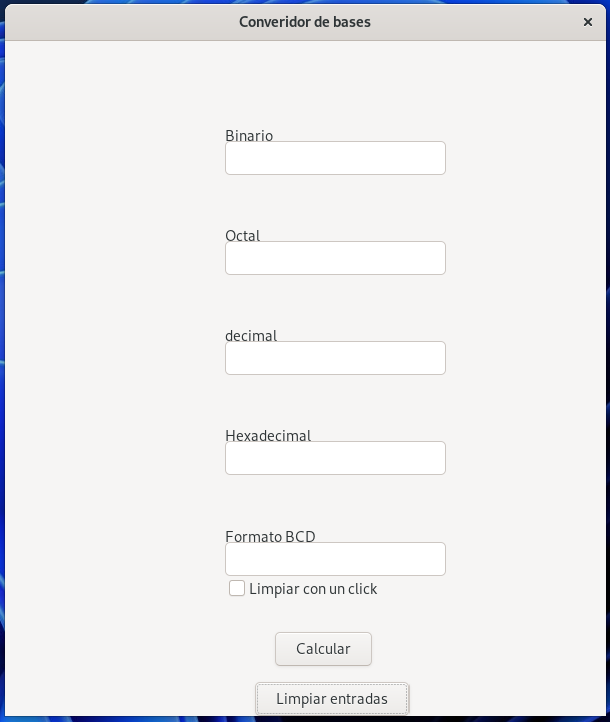
\includegraphics[width=7cm]{imag//ProgramDesign.png}
		\caption{Diseño del programa}
		% Convertidor
		\label{ProgramDesign}
		\end{center}
		%%\vspace{-1cm}
 		\end{figure}

		Para limpiar los campos de entrada de texto se crearon dos formas, una mediante
		un botón, y otra a través de un click sobre cualquiera de los campos. El cambio de 
		metodo se da a través de el check con la leyenda: Limpiar con un click.
		
		Para el proceso de conversión se existen muchas formas de realizarlo, sin embargo
		se observo que pasar de Decimal a Binario, Octal y Hexadecimal se debe dividir el número
		decimal entre la base solicitada e ir concatenando los modulos de cada divición
		hasta obtener cero, como se muestra en la figura \ref{decToOct}, dondé se convierte de decimal
		a octal.

		% Coloca imagen de diseño de imagen
		\begin{figure}[H]
		\begin{center}
		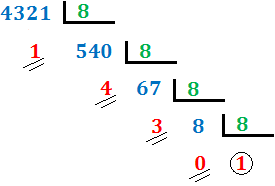
\includegraphics[width=7cm]{imag//decimalToOctal.png}
		\caption{Decimal a Octal}
		% Convertidor
		\label{decToOct}
		\end{center}
		%\vspace{-1cm}
		\end{figure}

		Con dicha forma de convertir las bases desde un número decimal se llego a un algoritmo el cual
		convierte desde decimal a octal, binario y Hexadecimal además de mostrar el resultado a el usuario
		y de forma opcional regresarlo mediante un return en caso de ser necesario, el cual se muestra en la 
		figura \ref{algDecToRest}.

		% Coloca imagen de diseño de imagen
		\begin{figure}[H]
			\begin{center}
			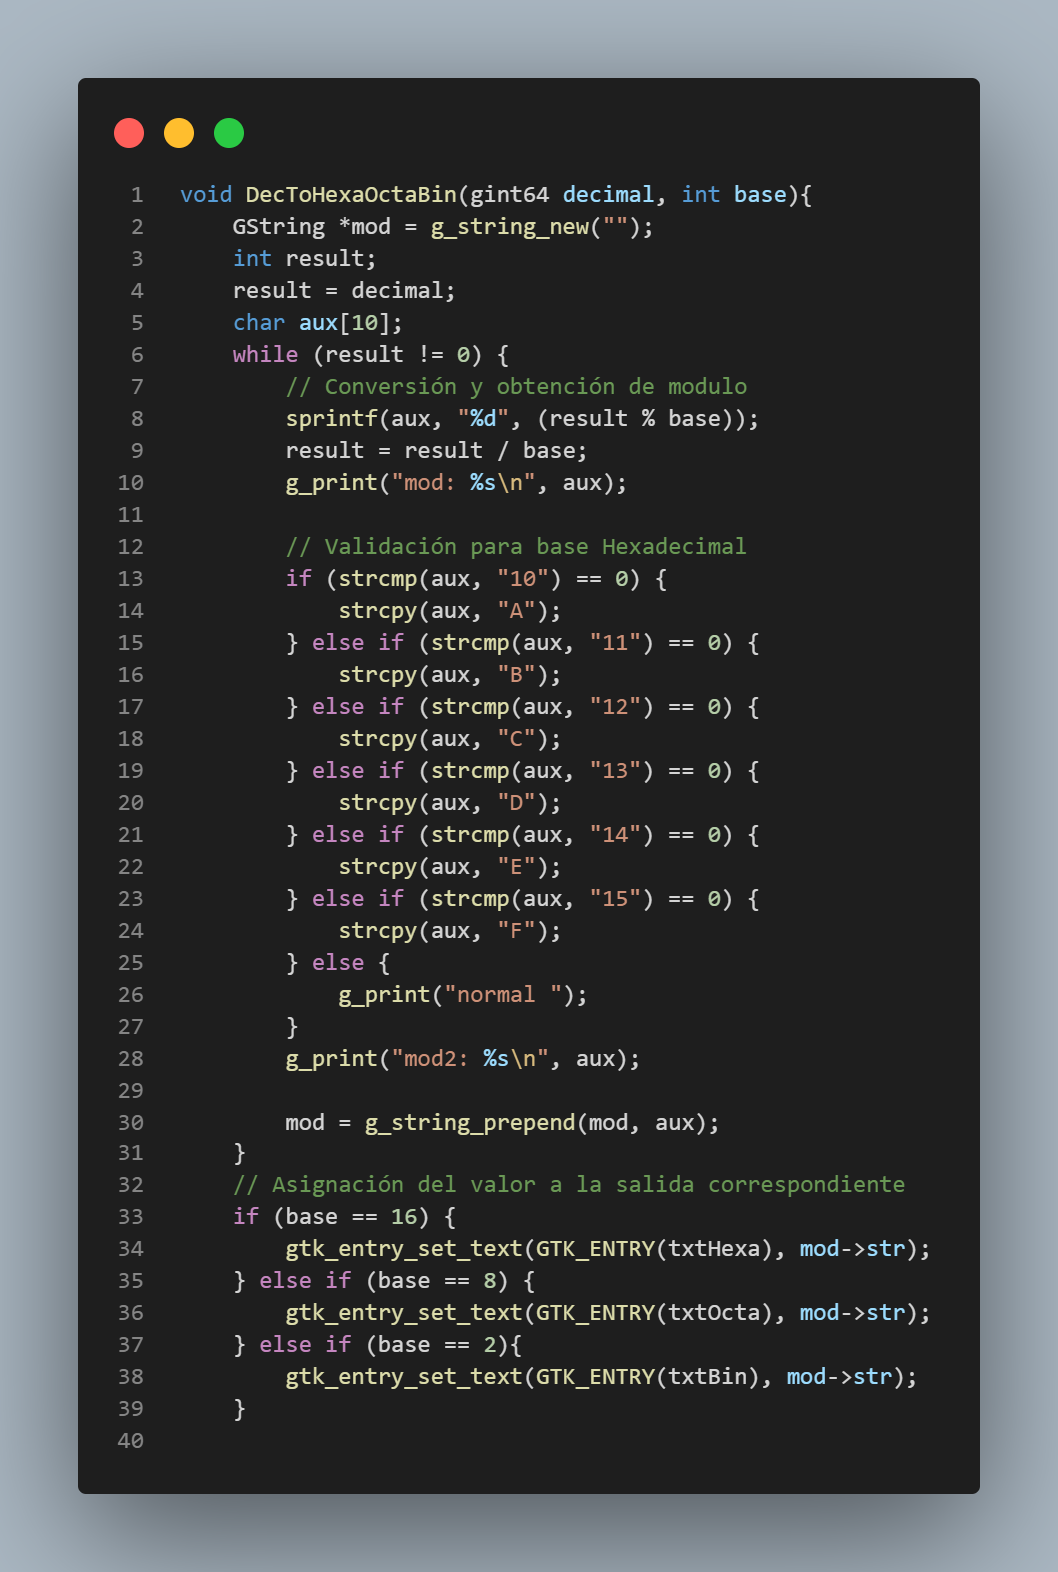
\includegraphics[width=10cm]{imag//algDecToRest.png}
			\caption{Algoritmo de conversión de bases}
			% Convertidor
			\label{algDecToRest}
			\end{center}
			%\vspace{-1cm}
			\end{figure}

			Con  el uso de este algoritmo solamente faltaría pasar de base Octal,
			Binario y Hexadecimal a binario, una vez echo esto el programa estaría
			casi completo, por lo que el primero en desarrollarse sera de Binario a 
			Decimal. Lo primero que se realizo fue buscar el punto decimal en la 
			cadena binaria para futuras versiones. En este caso solo nos centraremos
			en los numeros enteros. Una vez que tenemos una cadena binaria entera
			se recorre de derecha a izquierda para ir elevando la base a su potencia 
			correspodiente. Figura \ref{algBinToDec} 
			
			% Coloca imagen de diseño de imagen
			\begin{figure}[H]
			\begin{center}
			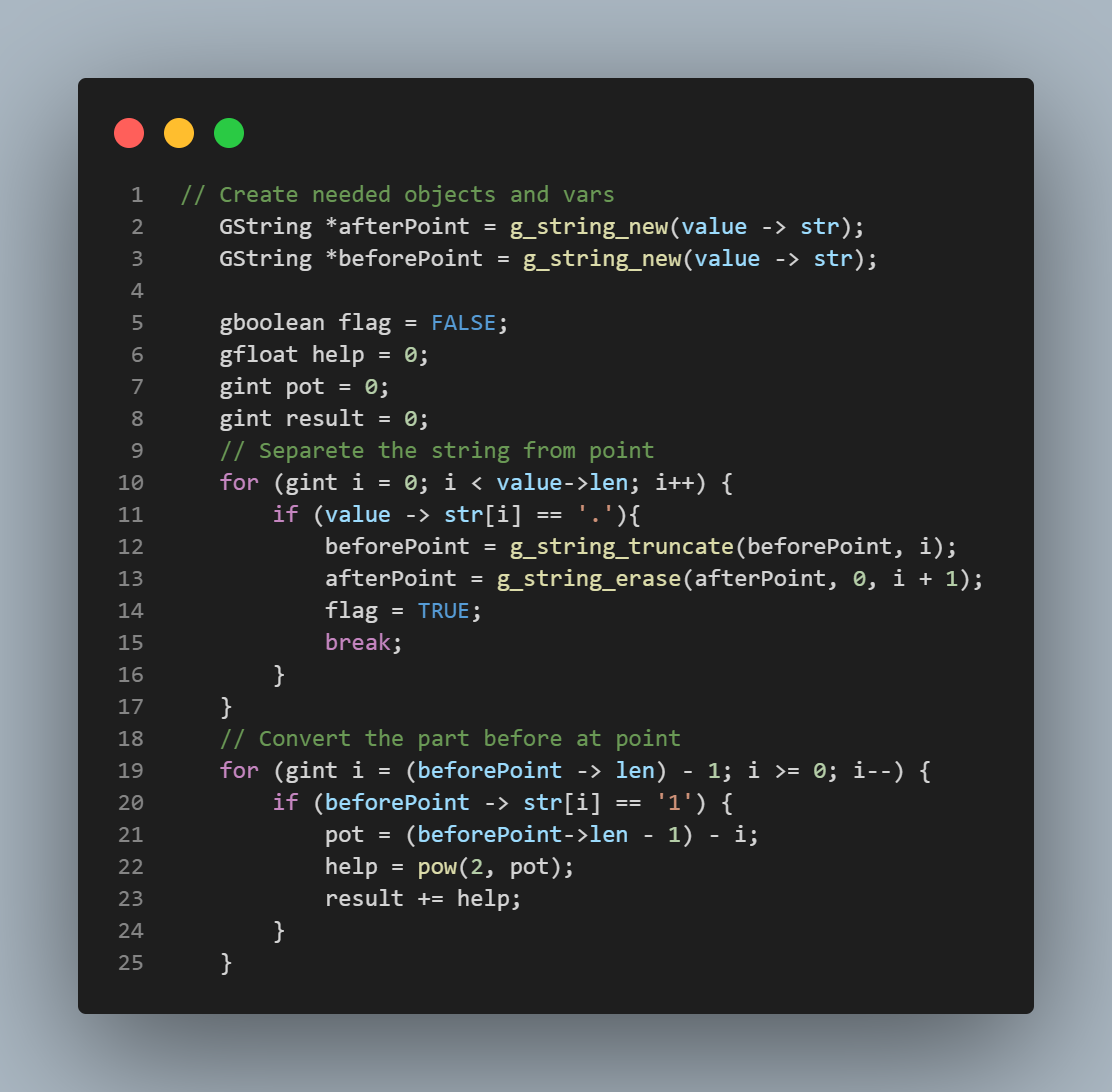
\includegraphics[width=10cm]{imag//algBinToDec.png}
			\caption{Algoritmo de binario a decimal}
			% Convertidor
			\label{algBinToDec}
			\end{center}
			%\vspace{-1cm}
			\end{figure}

			El resto de los algoritmos que convierten a binario se realizaron de forma similar. Una vez que fue
			posible convertir a decimal se utilizo el algoritmo de la figura \ref{algDecToRest} para llegar a las 
			demás bases.

			Para el formato BCD primero tenemos que tomar en cuenta que la cadena binaria se divide en grupos de 
			4 elementos para posteriormente transformarlos a decimal de forma separada y concatenar dichos numeros para 
			obtener el resultado.

			Se desarrollo un algoritmo que asegura que la cadena contendra grupos de 4 elementos, posteriormente utiliza 
			el mismo algoritmo de conversión de Binario a Decimal (figura \ref{algBinToDec}) por grupos de 4 en 4 elementos.
			Por ultimo concatena los resultados separados y muestra el resultado. Algoritmo en la figura \ref{algBcdToDec}.
			De forma adicional se transformo el formato bcd a Octal, Binario y Hexadecimal utilizando la funcion de la figura 
			\ref{algDecToRest} y el valor decimal obtenido.


			AGREGAR BASES A FORMATO BCD

			% Coloca alg de BCD a decimal
			\begin{figure}[H]
			\begin{center}
			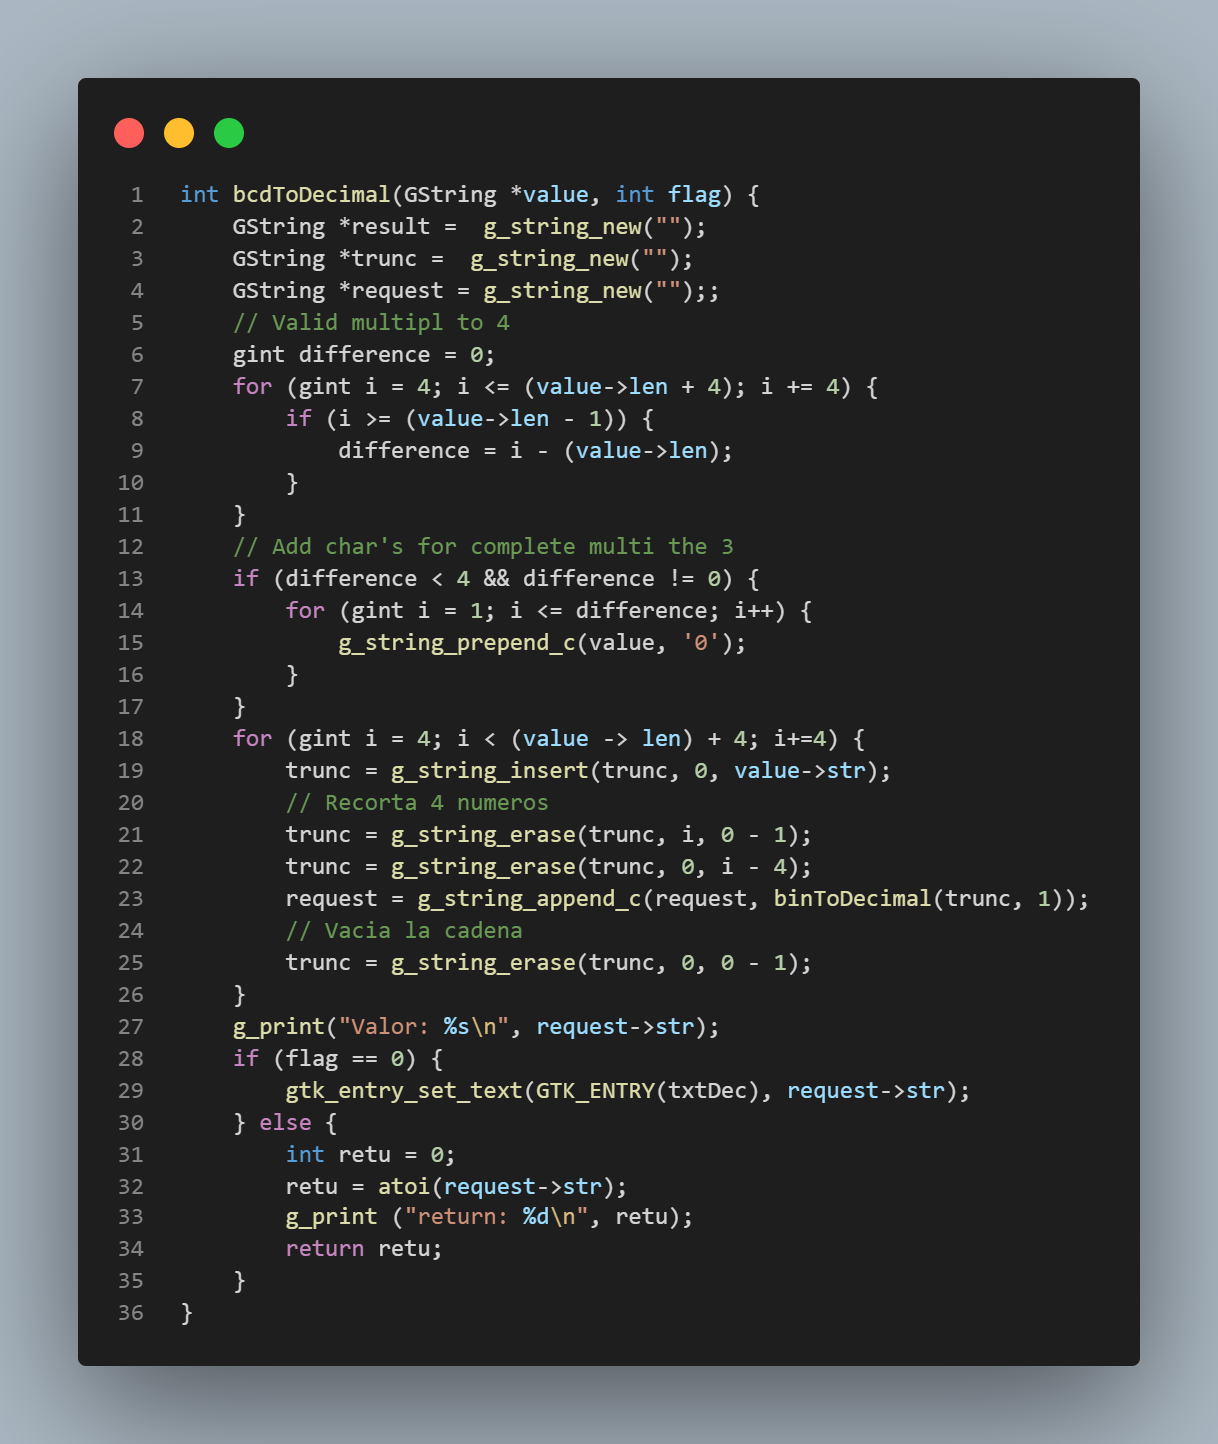
\includegraphics[width=10cm]{imag//algBcdToDec.png}
			\caption{Algoritmo de BCD a decimal}
			% Convertidor
			\label{algBcdToDec}
			\end{center}
			%\vspace{-1cm}
			\end{figure}
	
	\renewcommand{\labelenumi}{\arabic{enumi}.}
    
    	
    \section{Resultados}
		El programa actua según lo esperado, siendo capaz de convertir de cualquier base a el resto (dentro de las admitidas. Figura \ref{programFuntion}).
		Aún es posible mejorar el código utilizando otras herramientas que nos proveé C, además de agregar aperaciónes a el programa
		como lo son la suma, resta, etc. Pero dentro de lo esperado para este proyecto se cumplieron los Objetivos de la signación.
		
		% Coloca alg de BCD a decimal
		\begin{figure}[H]
		\begin{center}
		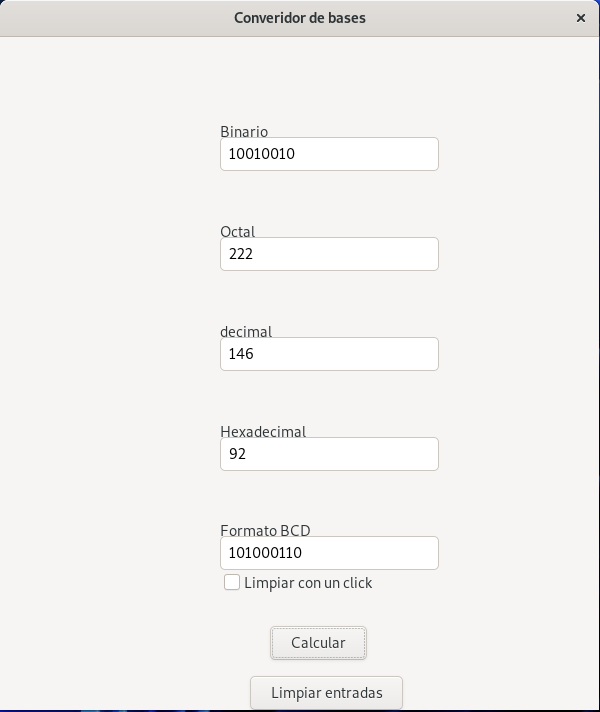
\includegraphics[width=10cm]{imag//programFuntion.png}
		\caption{Muestra de funcion del programa finalizado}
		% Convertidor
		\label{programFuntion}
		\end{center}
		%\vspace{-1cm}
		\end{figure}

	    
	    \section{Conclusiones}
		El programa se completo con exito, si bien no se realizaron conversiónes entre algunas bases
		de forma directa, el objetivo del programa es poder realizar el cambio de base de un numero de
		la manera más eficiente posible, que es lo que se realizo en dicho algoritmo, reciclar y generalizar
		un algoritmo para mejorar su legibilidad y eficiencia.
		
		Código fuente: \url{https://github.com/UnsisWorks/convert_base_gtk}
    
	\newpage
	
	% \section{Anexo de ecuaciones}
	
	% En caso des ser necesario se deben agregar ecuaciones que se hayan empleado

	% %Agrega todo lo ingresado tal cual
	% \begin{verbatim}
	% 	!"##$$%&%&/()
	% \end{verbatim}

	\cfoot{\LaTeX}
\end{document}